\section{Simulation of posterior distribution} \label{Appendix:Simulation}

% \begin{eqnarray}
% \mathbb P(\psi | \cdot) = C \cdot exp \left\{ -\frac{1}{2}(\psi'M\psi + 2\psi'N + C') \right\}
% \end{eqnarray}
% $\psi \sim N(-M^{-1}N,M^{-1})$

The Bayesian estimator uses the data augmentation approach \citep[proposed by][]{Albert1993} that treats the latent outcome and valuation variables as nuissance parameters.
The following four steps illustrate the first iteration of the estimator for the first-stage matching model. 

\subsection{Match valuations for unobserved groups}

The algorithm starts by simulating the latent match valuations for unobserved groups conditional on the data and parameters. In the first iteration illustrated here, the slope parameter alpha (blue asterisk) and the match valuations of the equilibrium groups (red asterisks) are initially set to zero and match valuations for unobserved groups (black circles) are drawn from a normal distribution with mean zero.
For the observed groups to be in equilibrium, the match valuation of the unobserved groups must be lower than the maximum equilibrium group valuation. The draws from the normal are therefore censored from above (gray shades).

\subsection{Match valuations for first observed group}


In the next step, the match valuation is drawn from a normal distribution with mean zero (conditional mean given by the dashed line). 
%In the first iteration, 
The equilibrium condition holds because the valuation of the second equilibrium group is larger than that of any non-equilibrium group (indicated by the yellow shades). Thus the valuation can be drawn from an uncensored normal. 
%In the second iteration, the draw from the normal is censored from below (grey shades) to guarantee an equilibrium valuation. 


\subsection{Match valuations for second observed group}

Same procedure as in step 2.


\subsection{Alpha slope parameter}

Fit a regression based on the given valuations and data (solid line) and draw alpha (dashed blue line) from a normal distribution with mean and standard deviation of the estimated slope parameter.
Use the new alpha draw in the next iteration to simulate the latent match valuations, etc etc.

\clearpage

\begin{table}[thbp!]
\caption{Simulation of posterior distribution: Conditional Draws for match valuations and model parameters}
\begin{center}
\begin{tabular}{lll}
1. Match valuations for unobserved groups & & 2. Match valuation for 1st observed group\\
before. \hfill after. & & before. \hfill after.\\
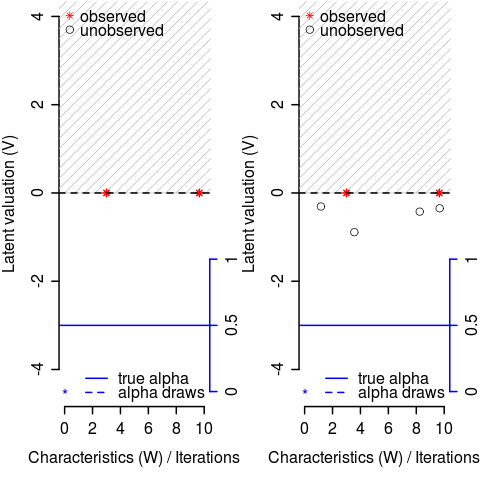
\includegraphics[width=0.45\textwidth]{./inputs/figures/Vunobs} & & 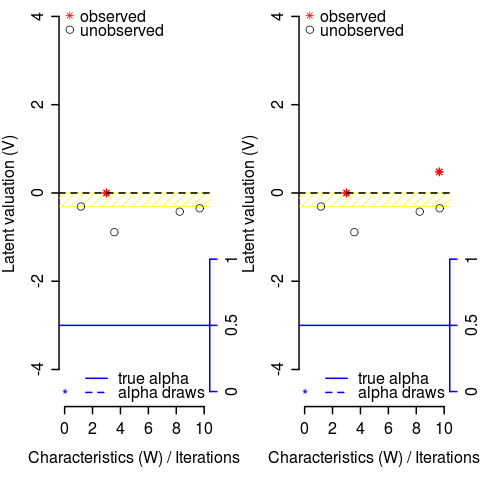
\includegraphics[width=0.45\textwidth]{./inputs/figures/Vobs1}\\
& & \\
\end{tabular}
\begin{tabular}{lll}
3. Match valuation for 2nd observed group & & 4. Alpha slope parameter\\
before. \hfill after. & & before. \hfill after.\\
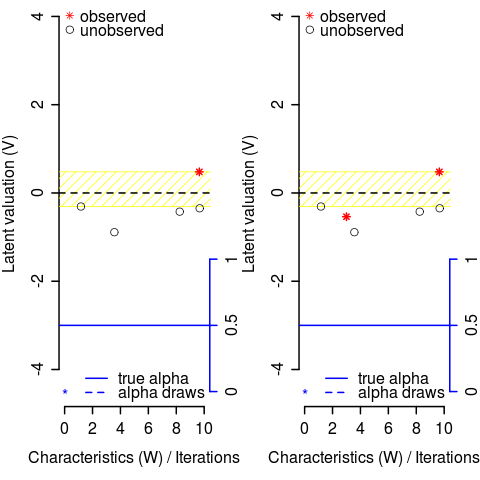
\includegraphics[width=0.45\textwidth]{./inputs/figures/Vobs2} & & 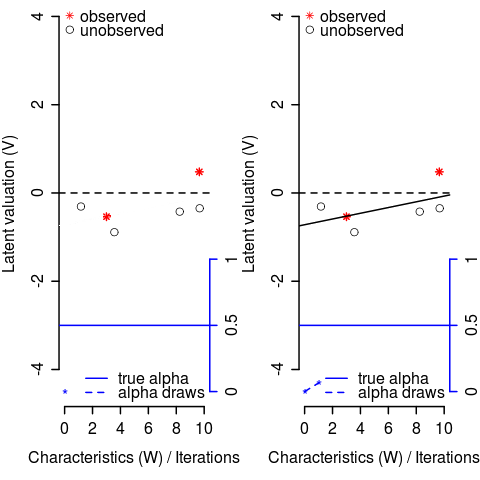
\includegraphics[width=0.45\textwidth]{./inputs/figures/alpha}
\end{tabular} 
\end{center}
\end{table}





